\apendice{Documentación de usuario}

\section{Introducción}
Esta parte del anexo define el proceso que debe seguir el usuario para poder visualizar el cuadro de mandos.

\section{Requisitos de usuarios}
Los requisitos de usuarios para visualizar el cuadro de mandos son los siguientes:
\begin{itemize}
    \item Disponer de un dispositivo electrónico con conexión a internet.
    \item Tener instalado un navegador web, con el que acceder a la url dónde está alojado el cuadro de mandos.
    \item Estar registrado en PowerBI con una cuenta de la UBU en la cual se ha solicitado un periodo de prueba o comprado PowerBI Pro. 
\end{itemize}

\section{Instalación}
Para visualizar el cuadro de mando, no va a tener que hacer ninguna instalación, solo tendría que descargar un navegador web en caso de no tenerlo ya instalado.

\section{Manual del usuario}
Para acceder al cuadro de mandos se debe ir al siguiente \href{https://app.powerbi.com/reportEmbed?reportId=1bac7505-a8ee-4592-81ea-4d9384ce787d&autoAuth=true&ctid=2aa3b0b5-a782-4f38-a898-e483b20e8d61&config=eyJjbHVzdGVyVXJsIjoiaHR0cHM6Ly93YWJpLW5vcnRoLWV1cm9wZS1yZWRpcmVjdC5hbmFseXNpcy53aW5kb3dzLm5ldC8ifQ\%3D\%3D}{enlace}.

\subsection{Inicio}
La hoja resumen es la primera página que se visualiza al entrar en el cuadro de mandos.

\begin{figure}[h]
    \advance\leftskip-0.5cm \rightskip5cm
    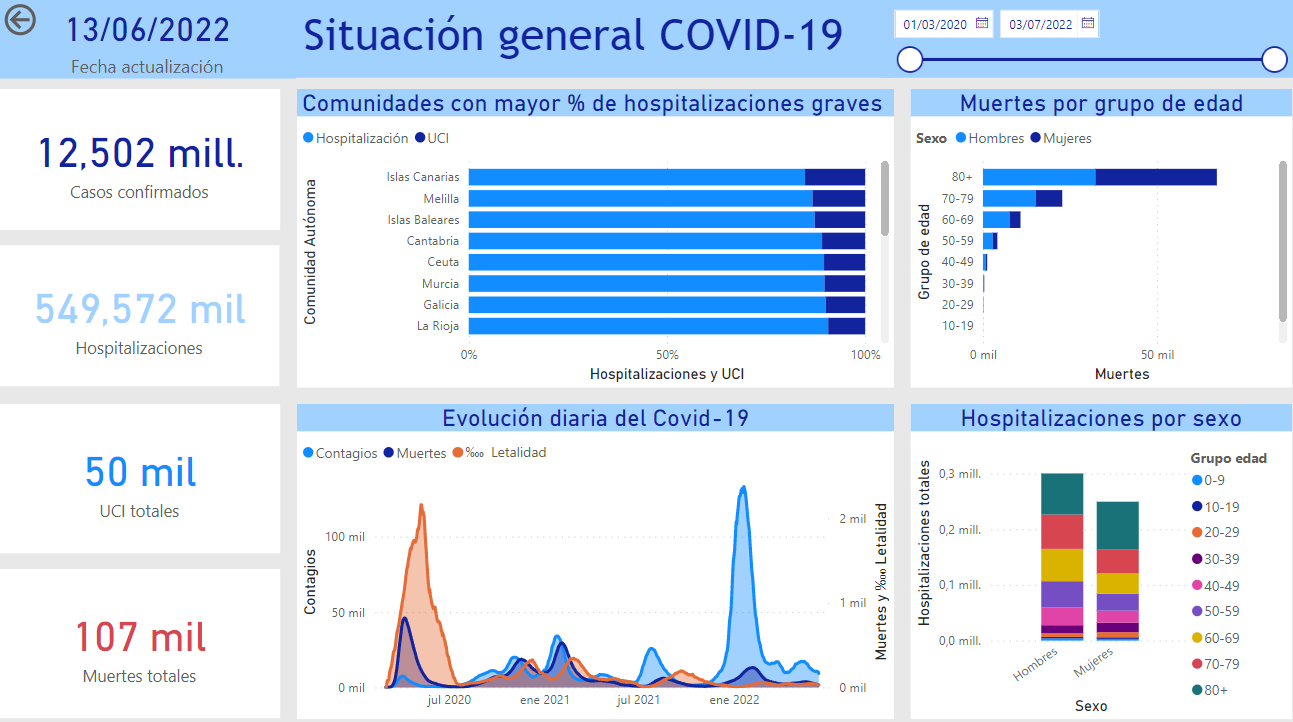
\includegraphics[scale=0.55]{img/powerBI_resumen.PNG}
    \caption{Resumen.}
\end{figure}

En ella se pueden visualizar diferentes etiquetas y gráficos que proporcionan información general de la situación de Covid-19.

\subsubsection{Fecha}
Dentro de esta página se permite la elección de la fecha en la que se quieren ver los datos.
Para ello, dispone de un calendario para elegir las fechas.
\imagen{info3_calen}{Calendario de selección de fechas.}


Otra forma que ofrece para la selección de fechas es mediante una barra que permite la misma funcionalidad que el calendario.
\imagen{info4-calen}{Barra de selección de fechas.}

\subsubsection{Información gráficos}
En cada gráfico se permite obtener información más específica colocando el cursor sobre cada gráfico en función de los datos que se quieran adquirir.
\imagen{info-1}{Información específica del gráfico de hospitalizaciones por sexo.}

\subsection{Incidencia acumulada}
La hoja incidencia acumulada es la segunda página que se visualiza al entrar en el cuadro de mandos.
\begin{figure}[h]
    \advance\leftskip0.5cm \rightskip5cm
    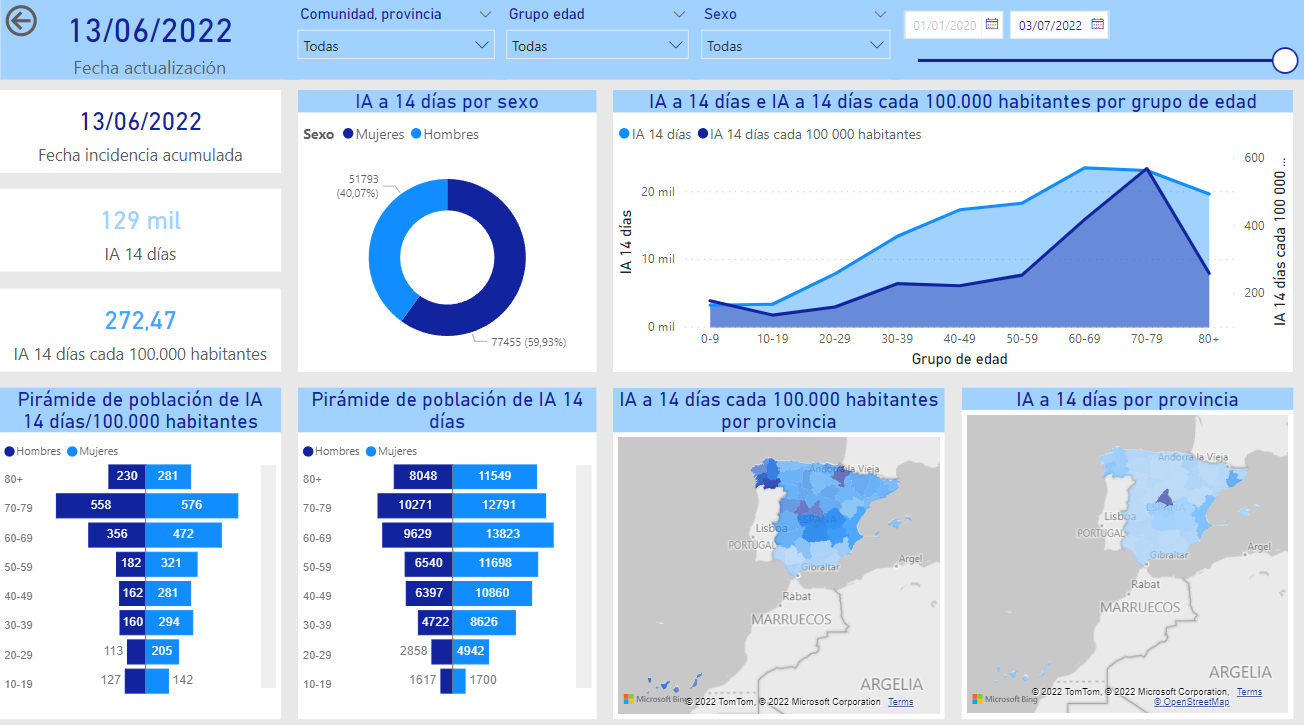
\includegraphics[scale=0.5]{img/powerBI_IA.PNG}
    \caption{Incidencia acumulada.}
\end{figure}
En ella se pueden visualizar diferentes etiquetas y gráficos que proporcionan información sobre la incidencia acumulada.
\newpage
\subsubsection{Fecha}
Dentro de esta página se permite la elección de la fecha en la que se quieren ver los datos.
Para ello, dispone de un calendario para elegir las fechas.
\imagen{info6_calen}{Calendario de selección de fechas.}

Otra forma que ofrece para la selección de fechas es mediante una barra que permite la misma funcionalidad que el calendario.
\imagen{info7_calen}{Barra de selección de fechas.}

\subsubsection{Filtros}
En esta página se permite el filtrado de la información mediante diversos filtros, entre los que se incluyen:
\begin{itemize}
    \item Filtrado por comunidades autónomas y provincias.
    \imagen{filtro-1}{Filtrado por comunidades autónomas y provincias.}
    \item Filtrado por grupo de edad.
    \imagen{filtro-2}{Filtrado por grupo de edad.}
    \item Filtrado por sexo
    \imagen{filtro-3}{Filtrado por sexo.}
\end{itemize}

\subsubsection{Información gráficos}
En cada gráfico se permite obtener información más específica colocando el cursor sobre cada gráfico en función de los datos que se quieran adquirir.
\imagen{info-5}{Información específica de IA a 14 días por sexo.}

\subsection{Casos y muertes}
La hoja casos y muertes es la tercera página que se visualiza al entrar en el cuadro de mandos.

\begin{figure}[h]
    \advance\leftskip-0.5cm \rightskip5cm
    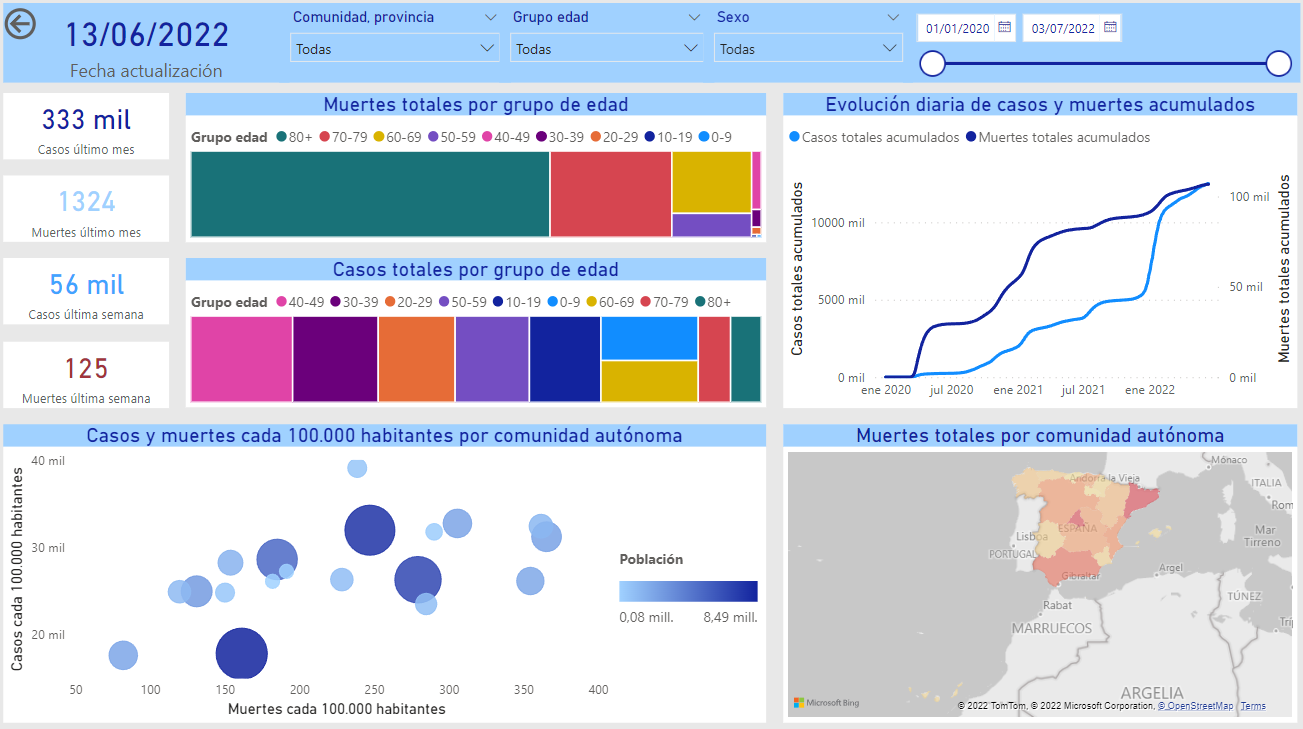
\includegraphics[scale=0.55]{img/powerBI_casosYmuertes.PNG}
    \caption{Casos y muertes.}
\end{figure}

En ella se pueden visualizar diferentes etiquetas y gráficos que proporcionan información sobre los casos y muertes.

\subsubsection{Fecha}
Dentro de esta página se permite la elección de la fecha en la que se quieren ver los datos.
Para ello, dispone de un calendario para elegir las fechas.
\imagen{info9_calen}{Calendario de selección de fechas.}

Otra forma que ofrece para la selección de fechas es mediante una barra que permite la misma funcionalidad que el calendario.
\imagen{info10_calen}{Barra de selección de fechas.}

\subsubsection{Filtros}
En esta página se permite el filtrado de la información mediante diversos filtros, entre los que se incluyen:
\begin{itemize}
    \item Filtrado por comunidades autónomas y provincias.
    \imagen{filtro-4}{Filtrado por comunidades autónomas y provincias.}
    \item Filtrado por grupo de edad.
    \imagen{filtro-5}{Filtrado por grupo de edad.}
    \item Filtrado por sexo
    \imagen{filtro-6}{Filtrado por sexo.}
\end{itemize}

\subsubsection{Información gráficos}
En cada gráfico se permite obtener información más específica colocando el cursor sobre cada gráfico en función de los datos que se quieran adquirir.
\imagen{info-8}{Información específica de la evolución diaria de casos y muertes acumulados.}

\subsection{Ingresos y altas hospitalarias}
La hoja ingresos y altas hospitalarias es la cuarta página que se visualiza al entrar en el cuadro de mandos.

\begin{figure}[h]
    \advance\leftskip-0.5cm \rightskip5cm
    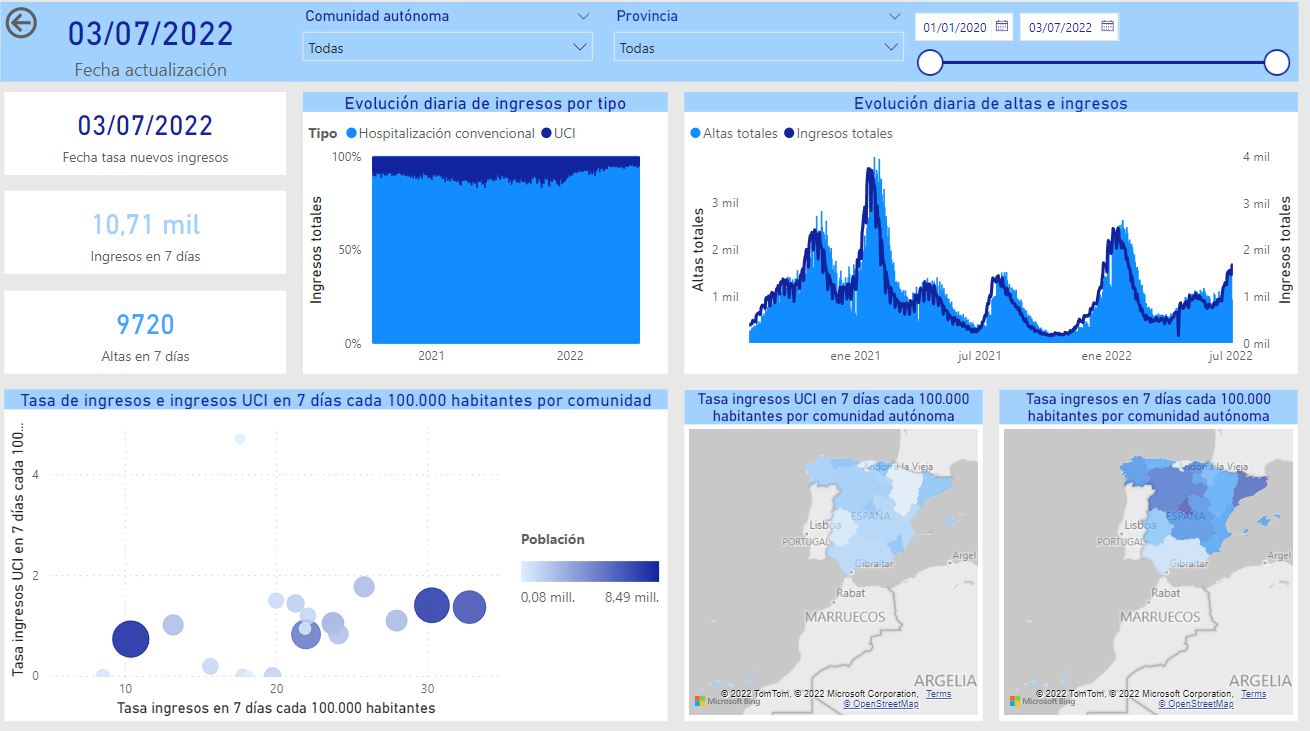
\includegraphics[scale=0.55]{img/powerBI_ingresosYaltas.PNG}
    \caption{Ingresos y altas hospitalarias.}
\end{figure}
\newpage

En ella se pueden visualizar diferentes etiquetas y gráficos que proporcionan información sobre los casos y muertes.

\subsubsection{Fecha}
Dentro de esta página se permite la elección de la fecha en la que se quieren ver los datos.
Para ello, dispone de un calendario para elegir las fechas.
\imagen{info11_calen}{Calendario de selección de fechas.}

Otra forma que ofrece para la selección de fechas es mediante una barra que permite la misma funcionalidad que el calendario.
\imagen{info12_calen}{Barra de selección de fechas.}

\subsubsection{Filtros}
En esta página se permite el filtrado de la información mediante diversos filtros, entre los que se incluyen:
\begin{itemize}
    \item Filtrado por comunidades autónomas.
    \imagen{filtro-7}{Filtrado por comunidades autónomas.}
    \item Filtrado por provincia
    \imagen{filtro-8}{Filtrado por provincia.}
\end{itemize}

\subsubsection{Información gráficos}
En cada gráfico se permite obtener información más específica colocando el cursor sobre cada gráfico en función de los datos que se quieran adquirir.
\imagen{info-9}{Información específica de la tasa de ingresos e ingresos UCI en 7 días cada 100.000 habitantes por comunidad.}


\subsection{Camas hospitalarias}
La hoja camas hospitalarias es la quinta página que se visualiza al entrar en el cuadro de mandos.

\begin{figure}[h]
    \advance\leftskip-0.5cm \rightskip5cm
    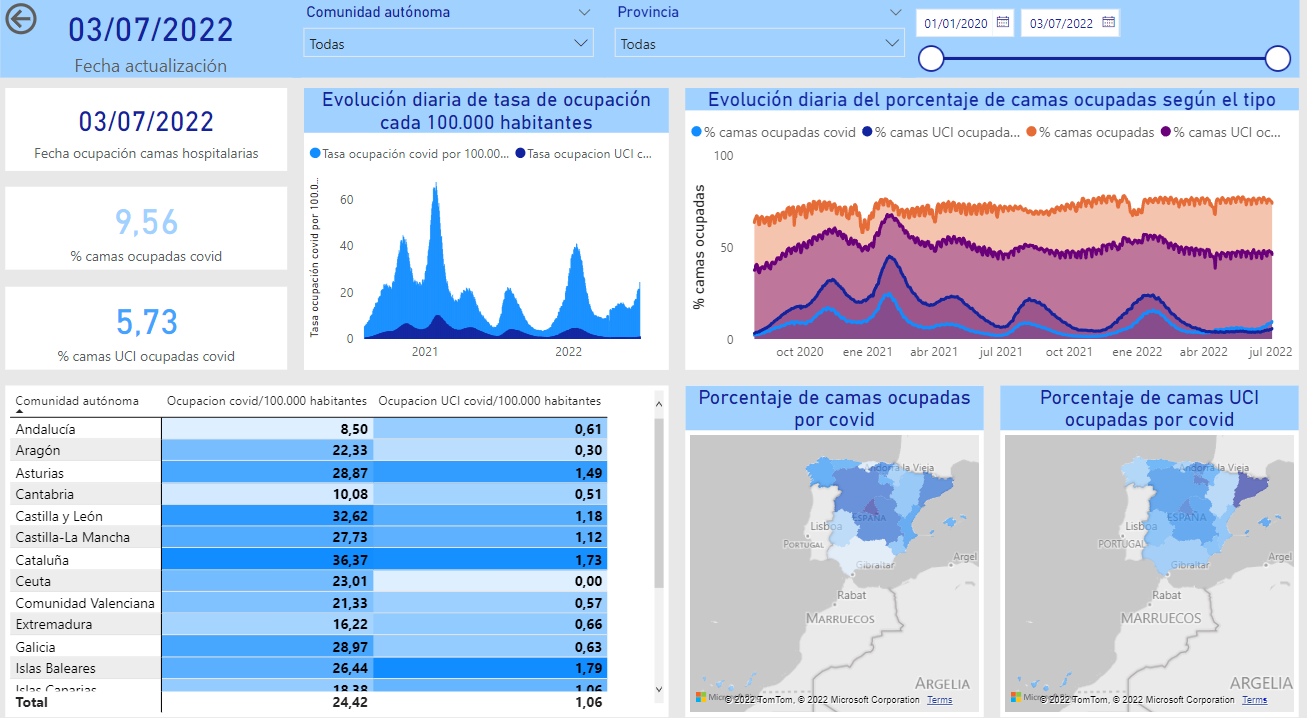
\includegraphics[scale=0.55]{img/powerBI_camas.PNG}
    \caption{Camas hospitalarias.}
\end{figure}

En ella se pueden visualizar diferentes etiquetas y gráficos que proporcionan información sobre los casos y muertes.

\subsubsection{Fecha}
Dentro de esta página se permite la elección de la fecha en la que se quieren ver los datos.
Para ello, dispone de un calendario para elegir las fechas.
\imagen{info13_calen}{Calendario de selección de fechas.}

Otra forma que ofrece para la selección de fechas es mediante una barra que permite la misma funcionalidad que el calendario.

\imagen{info14_calen}{Barra de selección de fechas.}

\subsubsection{Filtros}
En esta página se permite el filtrado de la información mediante diversos filtros, entre los que se incluyen:
\begin{itemize}
    \item Filtrado por comunidades autónomas.
    \imagen{filtro-9}{Filtrado por comunidades autónomas.}
    \item Filtrado por provincia
    \imagen{filtro-10}{Filtrado por provincia.}
\end{itemize}

\subsubsection{Información gráficos}
En cada gráfico se permite obtener información más específica colocando el cursor sobre cada gráfico en función de los datos que se quieran adquirir.

\imagen{info-10}{Información específica del porcentaje de camas UCI ocupadas por covid.}


\subsection{Residencias}
La hoja residencias es la sexta página que se visualiza al entrar en el cuadro de mandos.

\begin{figure}[h]
    \advance\leftskip0.35cm \rightskip5cm
    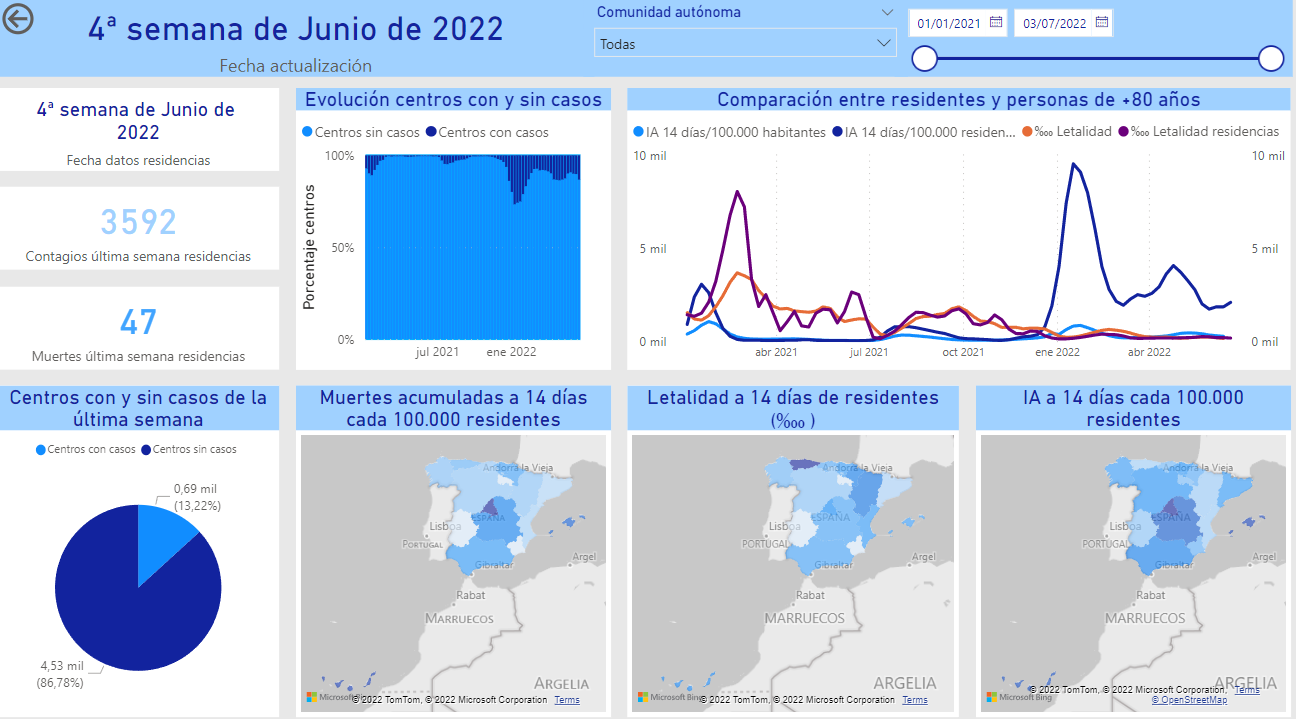
\includegraphics[scale=0.55]{img/powerBI_residencias.PNG}
    \caption{Residencias.}
\end{figure}
\newpage

En ella se pueden visualizar diferentes etiquetas y gráficos que proporcionan información sobre los casos y muertes.
\newpage
\subsubsection{Fecha}
Dentro de esta página se permite la elección de la fecha en la que se quieren ver los datos.
Para ello, dispone de un calendario para elegir las fechas.
\imagen{info15_calen}{Calendario de selección de fechas.}

Otra forma que ofrece para la selección de fechas es mediante una barra que permite la misma funcionalidad que el calendario.
\imagen{info16_calen}{Barra de selección de fechas.}

\subsubsection{Filtros}
En esta página se permite el filtrado de la información mediante diversos filtros, entre los que se incluyen:
\begin{itemize}
    \item Filtrado por comunidades autónomas.
    \imagen{filtro-11}{Filtrado por comunidades autónomas.}
\end{itemize}
\newpage
\subsubsection{Información gráficos}
En cada gráfico se permite obtener información más específica colocando el cursor sobre cada gráfico en función de los datos que se quieran adquirir.
\imagen{info-11}{Información específica de la comparación entre residentes y personas de +80 años.}